The methodology to study social and economic systems has been significantly influenced by the development of mathematical models that capture the essential features of these systems. In this chapter, we explore the transmission of ideas through social networks, differentiating between simple contagion, where ideas spread through brief, single exposures, with complex contagion, which requires multiple exposures or a significant number of early adopters to influence others. The chapter also delves into network theory fundamentals, discussing how the structure of networks affects the spread of ideas and behaviors. We describe two traditional threshold models and introduce topics such as the impact of bursty dynamics in human interactions and the concept of aging, highlighting how these factors influence the dynamics in social systems. These insights will be helpful to understand the results in the following chapters of the thesis.

\section{\label{sec:Introduction} Introduction}

The contagion of ideas is a process that has been studied for many years and is present in many social systems, ranging from small groups and communities to large networks and societies at a global scale. This process, often referred to as social contagion, involves the spread of ideas, behaviors, innovations, and emotions among individuals and groups through various forms of social interaction. The metaphor of contagion highlights the similarities between the spread of infectious diseases and the transmission of ideas, where a single "infected" individual can influence multiple others, leading to widespread adoption of new behaviors or beliefs.

In this context, binary-state models have emerged as a versatile tool to describe a variety of natural and social phenomena in systems formed by many interacting agents. Each agent is considered to be in one of two possible states: susceptible/infected, adopters/non-adopters, democrat/republican, etc., depending on the context of the model. The interaction among agents is determined by the underlying network and the dynamical rules of the model. Examples of binary-state models include processes of opinion formation \cite{Voter-original,sood-2005,fernandez-gracia-2014,redner-2019}, disease or social contagion \cite{granovetter-1978,pastor-satorras-2015}, among others. Extended and modified versions of these models can lead to very different dynamical behaviors than in the original model. As examples, the use of multi-layer  \cite{diakonova-2014,diakonova-2016,amato-2017} or time-dependent networks \cite{vazquez-2008}, higher-order interactions \cite{de-arruda-2020, iacopini-2019, cencetti-2021}, non-linear collective phenomena \cite{castellano-2009,peralta-2018}, noise \cite{carro-2016} and non-Markovian \cite{van-mieghem-2013,starnini-2017,peralta-2020A,chen-2020} effects induce significant changes to the dynamics.

With the advent of network theory and the increasing availability of large-scale data from online platforms, researchers have been able to study the contagion of ideas with unprecedented precision and detail. Duncan Watts and Steven Strogatz's small-world model \cite{watts1998collective} and Albert-László Barabási and Réka Albert's work on scale-free networks provided foundational insights into the structure of social networks and their role in facilitating or hindering the spread of information and ideas \cite{barabasi2009scale}.

Recent studies have focused on the mechanisms of social contagion in digital environments, where ideas can spread rapidly and widely through social media platforms \cite{online-platforms, jstor}. Analyses have identified emotional engagement and practical value as key drivers of sharing behavior \cite{ferrara-2015, steinert-2022}. Additionally, the role of social influence on online platforms has been explored, demonstrating how peer effects can significantly impact individuals' decisions to adopt new products or ideas \cite{jensen-2015}.

The contagion of ideas also plays a critical role in the diffusion of innovations. Rogger's seminal work outlines a theory of how, why, and at what rate new ideas and technology spread through cultures, highlighting the importance of social networks and opinion leaders in the spread of new ideas \cite{rogers2014}. Peer effects and social influence have been shown to play a significant role in the adoption of new technologies, with individuals more likely to adopt new products or services if they see others in their social network doing the same \cite{valente-1996, bollinger-2012}.

\section{\label{sec:Simple and Complex Contagion} Simple and Complex Contagion}

In the study of social contagion, researchers distinguish between two main types of contagion processes: simple contagion and complex contagion. Simple contagion refers to the spread of ideas, behaviors, or innovations primarily through single exposures or interactions, much like the transmission of infectious diseases. This process is characterized by the principle that an individual's likelihood of adopting a new idea or behavior increases with each additional exposure to that idea or behavior within their social network \cite{granovetter-1978,christakis2007spread, fowler2009cooperative}. In contrast, complex contagion involves multiple exposures or reinforcements from different sources within the network, often requiring a critical mass of adopters before an individual is influenced to adopt the idea or behavior \cite{centola-2007,centola-2010}.

\begin{figure}
    \centering
    \captionsetup{font=sf}
    \includegraphics[width=\textwidth]{Figs/Introduction/complex_simple.pdf}
    \caption[Simple and complex contagion processes]{Comparison between the different types of social interaction. {\bfseries Simple contagion}, where the agent considers just the pairwise interaction with one social contact (interaction highlighted with a dashed red line) and {\bfseries Complex contagion}, where the agent considers the interaction with multiple social contacts. There are two distinguishable types of Complex contagion: {\bfseries Multiple pairwise interactions}, where the agent considers the interaction with multiple social contacts (interactions highlighted with dashed red lines) and {\bfseries Higher-order interactions}, where the agent considers the interaction with a group of social contacts, all at once, in a single interaction (not pairwise). The green, yellow colors represent the state (idea, position, political party...). (The hypergraph representation is from Ref. \cite{de-arruda-2020}).}
    \label{fig:SimpleComplexContagion}
\end{figure}

Simple contagion is often described as a process that involves only dyadic interactions, where the adoption of an idea or behavior is facilitated by direct contact between two individuals. This type of contagion is fundamental to understanding how information, rumors, or diseases spread through populations via direct, pairwise connections \cite{pastor2001epidemic, newman2002spread}. The dynamics of simple contagion are crucial for the rapid dissemination of information and the efficient spread of both beneficial and detrimental behaviors across social ties \cite{christakis2007spread, fowler2009cooperative}.

In contrast, complex contagion occurs in scenarios where adoption is not merely a result of dyadic interactions but also involves group dynamics and the reinforcement from multiple sources within the network. This type of contagion often requires a critical mass or threshold of adopters within an individual's social network to trigger the adoption of the idea, behavior, or innovation \cite{centola-2007,centola-2010}. Granovetter's work on threshold models of collective behavior further illuminates this concept by exploring how individual thresholds for action or adoption depend on the proportion of others adopting the behavior, highlighting the nonlinear nature of social influence and the importance of group interaction in complex contagion processes \cite{granovetter-1978}.

The multiple exposure necessary that characterizes complex contagion can be understood in two ways: (i) as a reinforcement of the idea or behavior from multiple pairwise (dyadic) interactions \cite{centola-2007,centola-2010}, or (ii) as a reinforcement from multiple sources in a group interaction (higher-order interactions) \cite{iacopini-2019,de-arruda-2020,battiston-2021}. In the first case, the peer pressure, characteristic of complex contagion processes, is included into the model, which is designed to be used a simple network of dyadic social contacts. In the second case, the group interaction is included in the higher-order network, which is a more general representation of the social contacts, where the interactions are not restricted to dyads \cite{de-arruda-2020}. See Fig. \ref{fig:SimpleComplexContagion} for a graphical representation of the different types of social interactions.

Moreover, real-world processes are influenced not solely by either simple or complex contagion mechanisms but by a complex interaction between the two (Hybrid contagion). Such multifaceted interactions give rise to varied outcomes, including phenomena like criticality, tricriticality, and echo chambers \cite{min-2018,diaz-diaz-2022}, all of which profoundly affect how information is spread, how behaviors are adopted, and how collective actions are formed.

There have been attempt to extract the simple/complex nature of a process from real data. For example, by analyzing the correlation between the infection order of network nodes and their local topology, it is possible to infer the type of contagion process that is taking place \cite{cencetti-2023}. This approach relies on observing a single instance of spreading to classify the contagion as simple, threshold-driven, or influenced by higher-order interactions, without requiring extensive data or knowledge of the network's global structure. Nevertheless, the classification of contagion processes remains a challenging task, as the dynamics of social contagion are influenced by a multitude of factors and high-quality data related to the infection process is often scarce.

\section{\label{sec:Granovetter-Watts threshold model} Granovetter-Watts threshold model}

In this thesis, we focus on the dynamics of complex contagion driven by multiple interactions in a network of dyadic social contacts (no higher-order interactions). In particular, we focus on a particular category of complex contagion models called \textbf{threshold models}.

Threshold models represent a critical conceptual framework in understanding how individual behaviors aggregate to produce collective outcomes, especially in contexts where decisions are influenced by the actions of others \cite{granovetter-1973,granovetter-1978}. By defining a "threshold" — the point at which an individual's perception of the collective behavior of others prompts them to act — these models offer insights into the pivotal role of social influence and network structure in driving large-scale changes from small initial actions \cite{dodds-2004}. Rooted in the interdisciplinary nexus of sociology, economics, and network theory, these models illuminate the mechanics behind phenomena as diverse as social movements, technological adoption, market dynamics, and even cascading failures within infrastructures. All these phenomena share a common thread: the need for a critical mass of adopters or actors to trigger a collective response, a threshold that must be crossed to initiate a cascade of actions or behaviors \cite{centola-2007,centola-2010}.

When we talk about threshold models, the model that comes to our minds is the threshold mdoel introduced by Mark Granovetter in 1978 \cite{granovetter-1978}, highlighting how individuals' actions are influenced by the number of others participating in a behavior. In this model, each individual has a threshold that determines the number of neighbors they need to observe adopting a behavior before they themselves adopt it. This threshold can be interpreted as a measure of an individual's susceptibility to social influence, capturing the idea that some people are more likely to adopt a behavior if they see many others doing the same, while others may require more convincing or reinforcement before they act. Duncan J. Watts in 2002 \cite{watts-2002} built upon Granovetter's concept, applying mathematical analysis to explore the model within complex networks. His work, particularly on how minor initial actions can lead to large cascades, further elucidated the relationship between individual thresholds and network structures. This model, known as the Granovetter-Watts threshold model, has since become a cornerstone of research on social contagion and collective behavior, offering a powerful lens through which to study the dynamics of complex contagion in social networks.

\begin{figure}
    \centering
    \captionsetup{font=sf}
    \includegraphics[width=\textwidth]{Figs/Introduction/cascade_gleeson.pdf}
    \caption[Cascade diagram of the Granovetter-Watts model]{Average density $n$ of active nodes in a Poisson random graph of mean degree $z$ and uniform threshold value $R$  \textbf{(a)} and threshold distributed is Gaussian with mean $R$ and standard deviation $0.2$ \textbf{(b)} (from Ref. \cite{gleeson-2007}). Seed fraction is set $n_0 = 0.01$. Lines show approximations to the global cascade boundaries. The phase transition is discontinuous.}
    \label{fig:Cascade_gleeson}
\end{figure}

\begin{theorem}[Granovetter-Watts model]
    An individual time step of the model is defined as follows:
    \begin{enumerate}
        \item Each node $i$ has a threshold $R_i$.
        \item At each time step, a node $i$ is selected at random.
        \item If the fraction of active neighbors of $i$ is greater than $R_i$, then $i$ becomes active.
    \end{enumerate}
\end{theorem}

The Granovetter-Watts model exhibits a phase transition from a regime where the adoption is rare, where there are only small cascades and none of them is global, to a regime where the adoption is widespread, where there are large cascades that reach all the system. This phase transition is discontinuous \cite{watts-2002,gleeson-2007}, and it is characterized by a critical threshold value $R_c$ that separates the two regimes (refer to Fig. \ref{fig:Cascade_gleeson}). In the regime where the global cascades are rare, the system is in a supercritical state $R > R_c$, and the cascades are small and localized. In the regime where all the system reaches adoption, the system is in a subcritical state $R > R_c$, and the cascades are fast and global. The phase transition is driven by the interplay between the individual thresholds (homogeneous or heterogeneous) and the network structure, and it is a result of the collective dynamics of the system.

The exploration of this model has been widespread, encompassing studies on various types of networks including regular lattices and small-world networks \cite{centola-2007}, as well as on random graphs \cite{gleeson-2007}. It has also been examined within the contexts of networks with modular and community structures \cite{gleeson-2008}, networks that exhibit clustering \cite{hackett-2011,hackett-2013}, hypergraphs \cite{de-arruda-2020}, and networks characterized by homophily \cite{diaz-diaz-2022}, among others. In addition, the literature has expanded to cover the effects of varying the rules for adoption, such as incorporating social reinforcement across multiple layers \cite{chen-2018}, examining the influence of opinion leaders and initial seed size on the process \cite{liu-2018, singh-2013}, the introduction of on-off thresholds \cite{dodds-2013}, and analyzing the dynamics when simple contagions compete with complex ones \cite{czaplicka-2016, min-2018, diaz-diaz-2022}. Further, empirical data have been used to test the predictions of the Granovetter-Watts model, demonstrating its applicability across a wide range of real-world situations \cite{centola-2010, karimi-2013, karsai-2014, rosenthal-2015, karsai-2016, mnsted-2017, unicomb-2018, guilbeault-2021}.

\section{\label{sec:The Sakoda-Schelling model} The Sakoda-Schelling model}

\begin{figure}
    \centering
    \captionsetup{font=sf}
    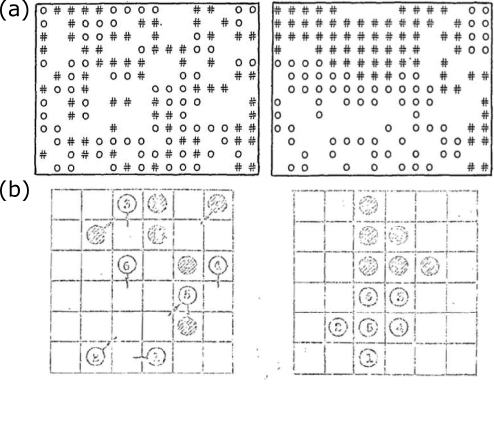
\includegraphics[width=0.7\textwidth]{Figs/Introduction/schelling_diagrams.png}
    \caption[Schelling and Sakoda checkerboard examples]{\textbf{(a)} Examples of the dynamics in Schelling's Segregation Model (from Schelling's original work \cite{Schelling}). \textbf{(b)} Examples of the dynamics in Sakoda’s Checkerboard Conceptual Model (from Sakoda's original work \cite{sakoda1949minidoka}).}
    \label{fig:Schelling_fig}
\end{figure}

Thomas C. Schelling's segregation model \cite{schelling-1969}, introduced in 1969, represents a key innovation in the use of agent-based modeling to explore social phenomena \cite{hegselmann-2017}. Schelling's model illustrates how individual preferences regarding neighbors can inadvertently lead to significant racial segregation in urban areas, even when these preferences are relatively mild. The model utilizes a checkerboard setup where each agent (representing a household) prefers to live in a neighborhood where at least a certain percentage of neighbors are of the same type (see Fig. \ref{fig:Schelling_fig}). Agents move to a new location if their tolerance threshold is not met. This simple rule leads to complex patterns, showing that even a slight preference for similar neighbors can result in highly segregated communities, an insight that has profound implications for understanding social dynamics and urban planning.

\begin{theorem}[Schelling's model]
    An individual time step of the model is defined as follows:
    \begin{enumerate}
        \item Each node $i$ has a tolerance threshold $T_i$.
        \item At each time step, a node $i$ is selected at random.
        \item If the fraction of different kind neighbors of $i$ is greater than $T_i$, then $i$ moves to a neighboring location where the fraction of different kind neighbors is less than $T_i$.
            \begin{itemize}
                \item If there is no available location, then $i$ remains in the same location.
            \end{itemize}
    \end{enumerate}
\end{theorem}

James M. Sakoda's model, initially conceptualized in his 1949 dissertation and fully introduced in Ref. \cite{sakoda1971checkerboard} pre-dates Schelling's work and offers a more nuanced approach to modeling social interactions using a similar checkerboard framework. Unlike Schelling's focus solely on segregation dynamics, Sakoda's model incorporates a broader range of social interactions by allowing agents to exhibit positive, neutral, or negative attitudes towards their neighbors. These attitudes influence the agents' movements across the board, aiming to optimize their local environment according to specific utility functions that aggregate the effects of surrounding agents. Sakoda's model is capable of simulating a variety of social phenomena beyond segregation, such as the formation of stable social clusters and the dynamics of group interactions \cite{hegselmann-2017}. 

Both models employ a checkerboard as the computational space where agents (or tokens) reside and interact according to predefined rules. The ``hand-made'' simulations performed by Sakoda and Schelling using a checkerboard discrete representation has since become a standard framework for studying agent-based models in social systems \cite{hegselmann-2017}. The checkerboard structure allows for the exploration of local interactions and the emergence of global patterns, providing a powerful tool for understanding the dynamics of social systems.

\begin{theorem}[Sakoda's model]
    An individual time step of the model is defined as follows:
    \begin{enumerate}
        \item Each node $i$ has an attitude matrix $A_i$.
        \item At each time step, a node $i$ is selected at random.
        \item $i$ evaluates the total utility for each neighboring location based on the sum of influences from all other agents on the board, weighted by distance.
        \item $i$ moves to the location with the highest utility.
        \begin{itemize}
            \item If there is no available location, then $i$ remains in the same location.
        \end{itemize}
    \end{enumerate}
\end{theorem}

The results of the Schelling's model demonstrated how even mild personal preferences can unexpectedly lead to significant societal segregation. Its insights have been applied across economics, sociology, urban planning, and complexity science, profoundly influencing both academic research and practical policy discussions. Schelling's model became a foundational example in agent-based modeling, helping to educate countless researchers and practitioners about the impact of individual actions on broader social patterns. This contribution was one of the key reasons Schelling was awarded the Nobel Prize in Economics in 2005, underscoring the model's enduring influence and importance. Nevertheless, when we check the update rules, we observe that the Schelling's model is a particular case of the previous Sakoda's model, where agents have a negative attitude towards different-kind agents and a fixed tolerance threshold. To honor the original contributions of both authors, we refer to this model as the Sakoda-Schelling model.

In particular, the Sakoda-Schelling model has been studied from a Statistical Physics point of view due to its close relation to different forms of Kinetic Ising-like models \cite{stauffer-2007,stauffer-2013}, and also addressing general questions of clustering and domain growth phenomena, as well as for the existence of phase transitions from segregated to non-segregated phases. For example, the relation with phase separation in binary mixtures has been considered \cite{Dall_Asta_2008,Vinkovic}, as well as the connection with the phase diagram of spin-1 Hamiltonians \cite{BEG,BlumeCapel,Gauvin_2009,Gauvin_2010}. In this context a useful classification of models is to distinguish between two possible types of dynamics \cite{Dall_Asta_2008}: ``constrained'', where agents just move to satisfying vacancies (if possible), and ``unconstrained'',  where agents' motion does not prevent them to remain unsatisfied. In addition, the motion can be short-range (only to neighboring sites, as in the original model) or long-range. Constrained motion has been named ``solid-like'' because it generally leads to frozen small clusters, while unconstrained motion has been considered ``liquid-like'' because it allows for large growing clusters \cite{Vinkovic}. Including the motion of satisfied agents leads to a noisy effect playing the role of temperature in a statistical physics approach. 

\section{\label{sec:Theoretical Framework} Theoretical Framework}

To explain the emergent properties exhibited by the agent based models and simulations, we need to develop a theoretical framework that captures the essential features of the system. This framework should provide a mathematical description of the dynamics, allowing us to analyze the system's behavior and predict its evolution over time. In the context of social contagion and collective behavior, the theoretical framework typically involves a set of differential equations or master equations that describe the evolution of the system's state variables.

The theoretical framework for agent-based models can be broadly classified into two main categories: mean-field approaches and network-based approaches \cite{barrat-2008}. Mean-field approaches treat the system as a homogeneous entity, where each agent interacts with the average behavior of the entire population. These approaches are well-suited for capturing the macroscopic dynamics of the system and are particularly useful for understanding the collective behavior that emerges from individual interactions. Network-based approaches, on the other hand, explicitly model the interactions between agents as a network structure, where nodes represent agents and edges represent interactions between them. These approaches are valuable for capturing the influence of the underlying network structure on the system's dynamics and for studying the impact of network properties on the spread of information and ideas.

\subsection{\label{sec:Approximate Master Equation} Approximate Master Equation}

A general framework for binary-state models in complex networks was developed by J. P. Gleeson \cite{gleeson-2011,gleeson-2013}, which provides a general set of differential equations, the Approximate Master Equation (AME), to describe the dynamics of any Markovian binary-state model on a network. This framework has been widely used to study the dynamics of social contagion, opinion formation, and other collective behaviors in complex networks. The framework allows for the analysis of the system's behavior, including the identification of phase transitions, the calculation of critical thresholds, and the prediction of the final state of the system \cite{gleeson-2013}.

To understand the AME, consider a node $i$ with a degree $k$ (i.e., $k$ connections to other nodes). Let $ m$ be the number of neighbors of $i$ that are in state $-1$ (e.g., 'infected'). If node $i$ is in state $+1$ (e.g., 'susceptible'), the rate \( T^{+}_{k,m} \) defines the probability per unit time that \( X \) will switch to state $-1$. Similarly, \( T^{-}_{k,m} \) defines the probability per unit time for a node in state '1' to switch to state $+1$. These rates are functions of both the degree \( k \) and the number \( m \) of neighbors in state $-1$, reflecting how the local network configuration influences state transitions.

Here is a basic representation of the mathematical framework used in the AME:
\begin{equation}
    \frac{d}{dt} x^{\pm}_{k,m} = -T^{\pm}_{k,m} x^{\pm}_{k,m} + T^{\mp}_{k,m} x^{mp}_{k,m} - (k-m) \beta^{\pm} x^{\pm}_{k,m} + (k-m+1) \beta^{\pm} x^{\pm}_{k,m-1} - m \gamma^{\pm} x^{\pm}_{k,m} + (m+1) \gamma^{\pm} x^{\pm}_{k,m+1}
\end{equation}

Here, $x^{+}_{k,m}$ and $x^{-}_{k,m}$ represent the fractions of nodes with degree \( k \) and \( m \) infected neighbors that are in state $+1$ and $-1$, respectively. $\beta^{\pm}$ and $\gamma^{\pm}$ are rates that describe how the infection spreads and recedes across the edges of the network, encapsulating the network's dynamic connectivity and its influence on the spread of states (see details in Ref. \cite{gleeson-2013})

A key advantage of the AME is its ability to capture the complex dynamics of networks by considering the interactions between neighboring nodes, making it more accurate than simpler models like the mean-field theory, which assumes independence between nodes. Moreover, from the AME, one can make approximate the shape of the solutions $x^{\pm}_{k,m} (t)$ to reduce the number of differential equations, recovering the pair approximation and the heterogeneous mean field \cite{gleeson-2013}.

On the other hand, the AME assumes a tree-like structure with negligible levels of clustering. This assumption implies that there are very few short loops in the network. This tree-like assumption simplifies the calculation and application of the AME by reducing the network's complexity, and becomes very useful for networks generated with the configuration model \cite{newman-book}, with any given degree distribution, at the limit $N \to \infty$.

Another limitation is based on the AME formulation itself, since framework is built assuming binary-state Markovian dynamics, which may not always accurately capture the real-world dynamics of social contagion. In fact, in next section, we will introduce the concept of bursty human dynamics, which is a non-Markovian effect that can significantly impact the dynamics of social contagion processes.

\section{\label{sec: Bursty Human Dynamics} Bursty Human Dynamics}

Bursty behavior refers to the irregular and sporadically timed patterns of interactions that include natural phenomena, like earthquakes and neuron firing, as well as human activities, such as email communication, mobility, and social dynamics. This section delves into the characteristics of bursty behavior, highlighting by empirical evidence, and discusses its significant implications for modeling human behavior.

Human activities often exhibit complex temporal patterns characterized by bursts---short periods of high activity interspersed with longer periods of inactivity (see examples Fig. \ref{fig:bursty_human_dynamics}(a-c)). This non-Poissonian behavior, referred to as burstiness, manifests across diverse human-driven processes and is extensively documented in communication dynamics, web browsing habits, and social interactions \cite{Barabasi2005Bursts, Vazquez2006Bursts}. The seminal work, by A. L. Barabási \cite{Barabasi2005Bursts}, highlighted the nature of email communications, where activity periods do not follow a regular pattern but are clustered in bursts. This phenomenon has since been observed universally across various platforms such as mobile phone calls, text messaging and social media \cite{karsai-2011, Miritello2013Capacity,moro,artime-2017,rybski-2012,zignani-2016,kumar-2020,iribarren-2009}.

Further research has analyzed temporal patterns, focusing on the persistence and periodicity of human interactions \cite{Clauset2007Proximity} or the effects of circadian rhythms \cite{Jo2012Circadian}, and has extended these analyses to web activity to predict behaviors across different online platforms \cite{Radicchi2009WebActivity}.

An important aspect of bursty dynamics is the distribution of inter-event times, which often exhibits heavy-tailed behavior, indicating that the probability of short inter-event times is higher than expected from a Poisson process (see Fig. \ref{fig:bursty_human_dynamics}(c)). As a result of this bursty human behaviour, there is an emergence of heterogeneus degree distributions \cite{Muchnik2013PowerLaw}, which have been observed in many social systems \cite{barabasi2009scale}. Further insights into the impact of burstiness on system dynamics come from studies linking it to memory and the structured nature of human dialogues, enhancing our understanding of how past interactions influence future activities \cite{karsai2012universal, Goh2008Burstiness, Eckmann2004Entropy}.

\begin{figure}
    \centering
    \captionsetup{font=sf}
    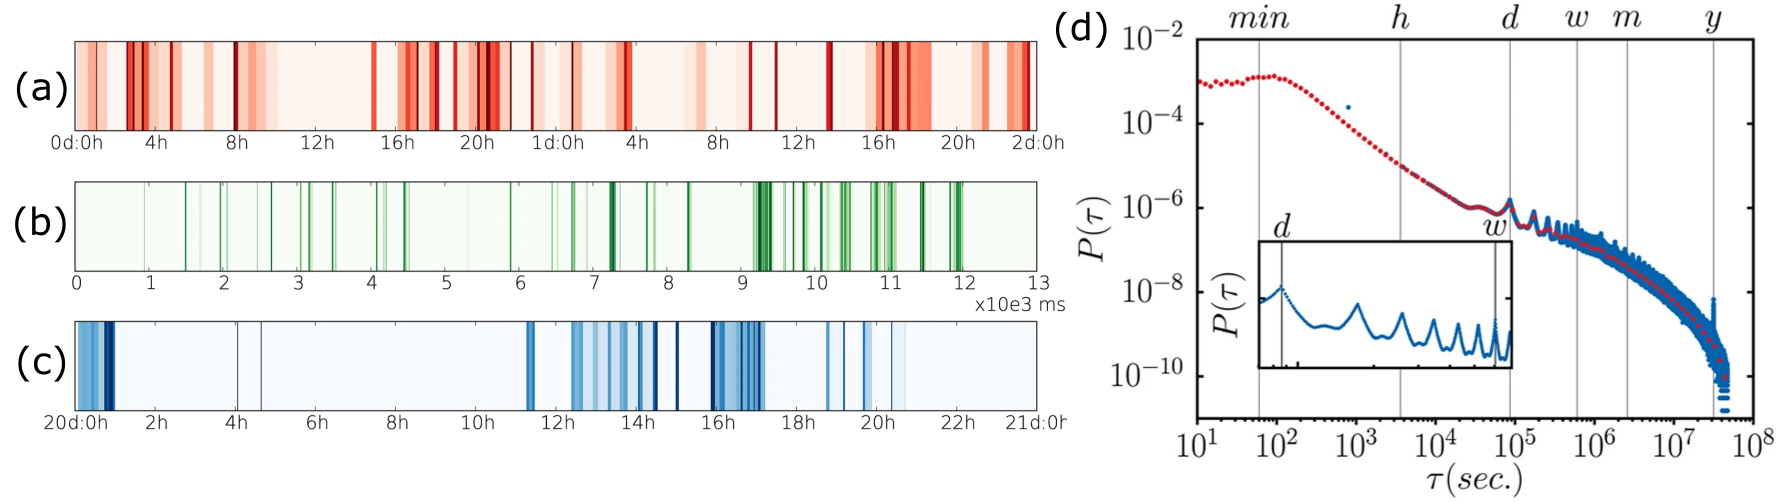
\includegraphics[width=\textwidth]{Figs/Introduction/bursty.png}
    \caption[Bursty human dynamics: examples and distribution]{\textbf{(a)} Sequence of earthquakes with magnitude larger than two at a single location (South of Chishima Island, 8th–9th October 1994). \textbf{(b)} Firing sequence of a single neuron (from rat's hippocampal). \textbf{(c)} Outgoing mobile phone call sequence of an individual. Shorter the time between the consecutive events darker the color (From Ref. \cite{karsai2012universal}). \textbf{(d)} Distribution of inter-event times for Twitter users. Blue and red dots represent the lin- and log-binned scales in the $\tau$ axis. The localized maxima in the tail of the distribution correspond to circadian rhythms, as shown in the bottom inset  (from Ref. \cite{artime-2017}). The distribution is heavy-tailed, indicating bursty behavior.}
    \label{fig:bursty_human_dynamics}
\end{figure}

Traditional models based on Poisson processes are often inadequate for capturing the real dynamics of human interactions due to the assumption of constant rates. To address these shortcomings, non-Poissonian models have been developed, which provide a better fit for empirical observations \cite{Vazquez2006Bursts}. We differentiate two main approaches to modeling bursty human dynamics:

\begin{itemize}
    \item \textbf{Activity-driven models (nodes activate):} These models incorporate the temporal aspects of human activity by assigning activity potentials to nodes within a network, dictating the likelihood of interactions based on observed human activity patterns \cite{Perra2012ActivityDriven}.
    \item \textbf{Temporal networks (links activate):} These models incorporate time-stamped interactions, allowing for an in-depth study of temporal patterns and the impact of burstiness on overall network dynamics \cite{Holme2012Temporal}.
\end{itemize}

While both approaches have been successful in capturing bursty human dynamics, they offer different perspectives on the underlying mechanisms driving these behaviors: activity-driven models emphasize the burstiness of individual attempts to interact with others, while temporal networks focus on the burstiness of the interactions themselves. The choice of model depends on the specific research question and the level of detail required to capture the dynamics of interest.

The implications of bursty behavior are profound, influencing the dynamics of network processes such as the spread of epidemics and information diffusion \cite{Rocha2013Bursts, Wang2009Viruses}. Understanding these dynamics aids in the design of better communication strategies and the improvement of technological infrastructures, aligning them more closely with natural human activity patterns.

\section{\label{sec:Aging mechanism} Aging mechanism}

"Aging" is one form of memory effect on which the rate of interactions depends on the persistence time of an agent in a state, modifying the transition to a different state \cite{fernandez-gracia-2011,perez-2016,boguna-2014}. This concept of aging, or "social inertia" \cite{Stark2008}, constrains the transitions in a way that the longer an agent remains in a given state, the smaller the probability to change it.

\begin{figure}
    \centering
    \captionsetup{font=sf}
    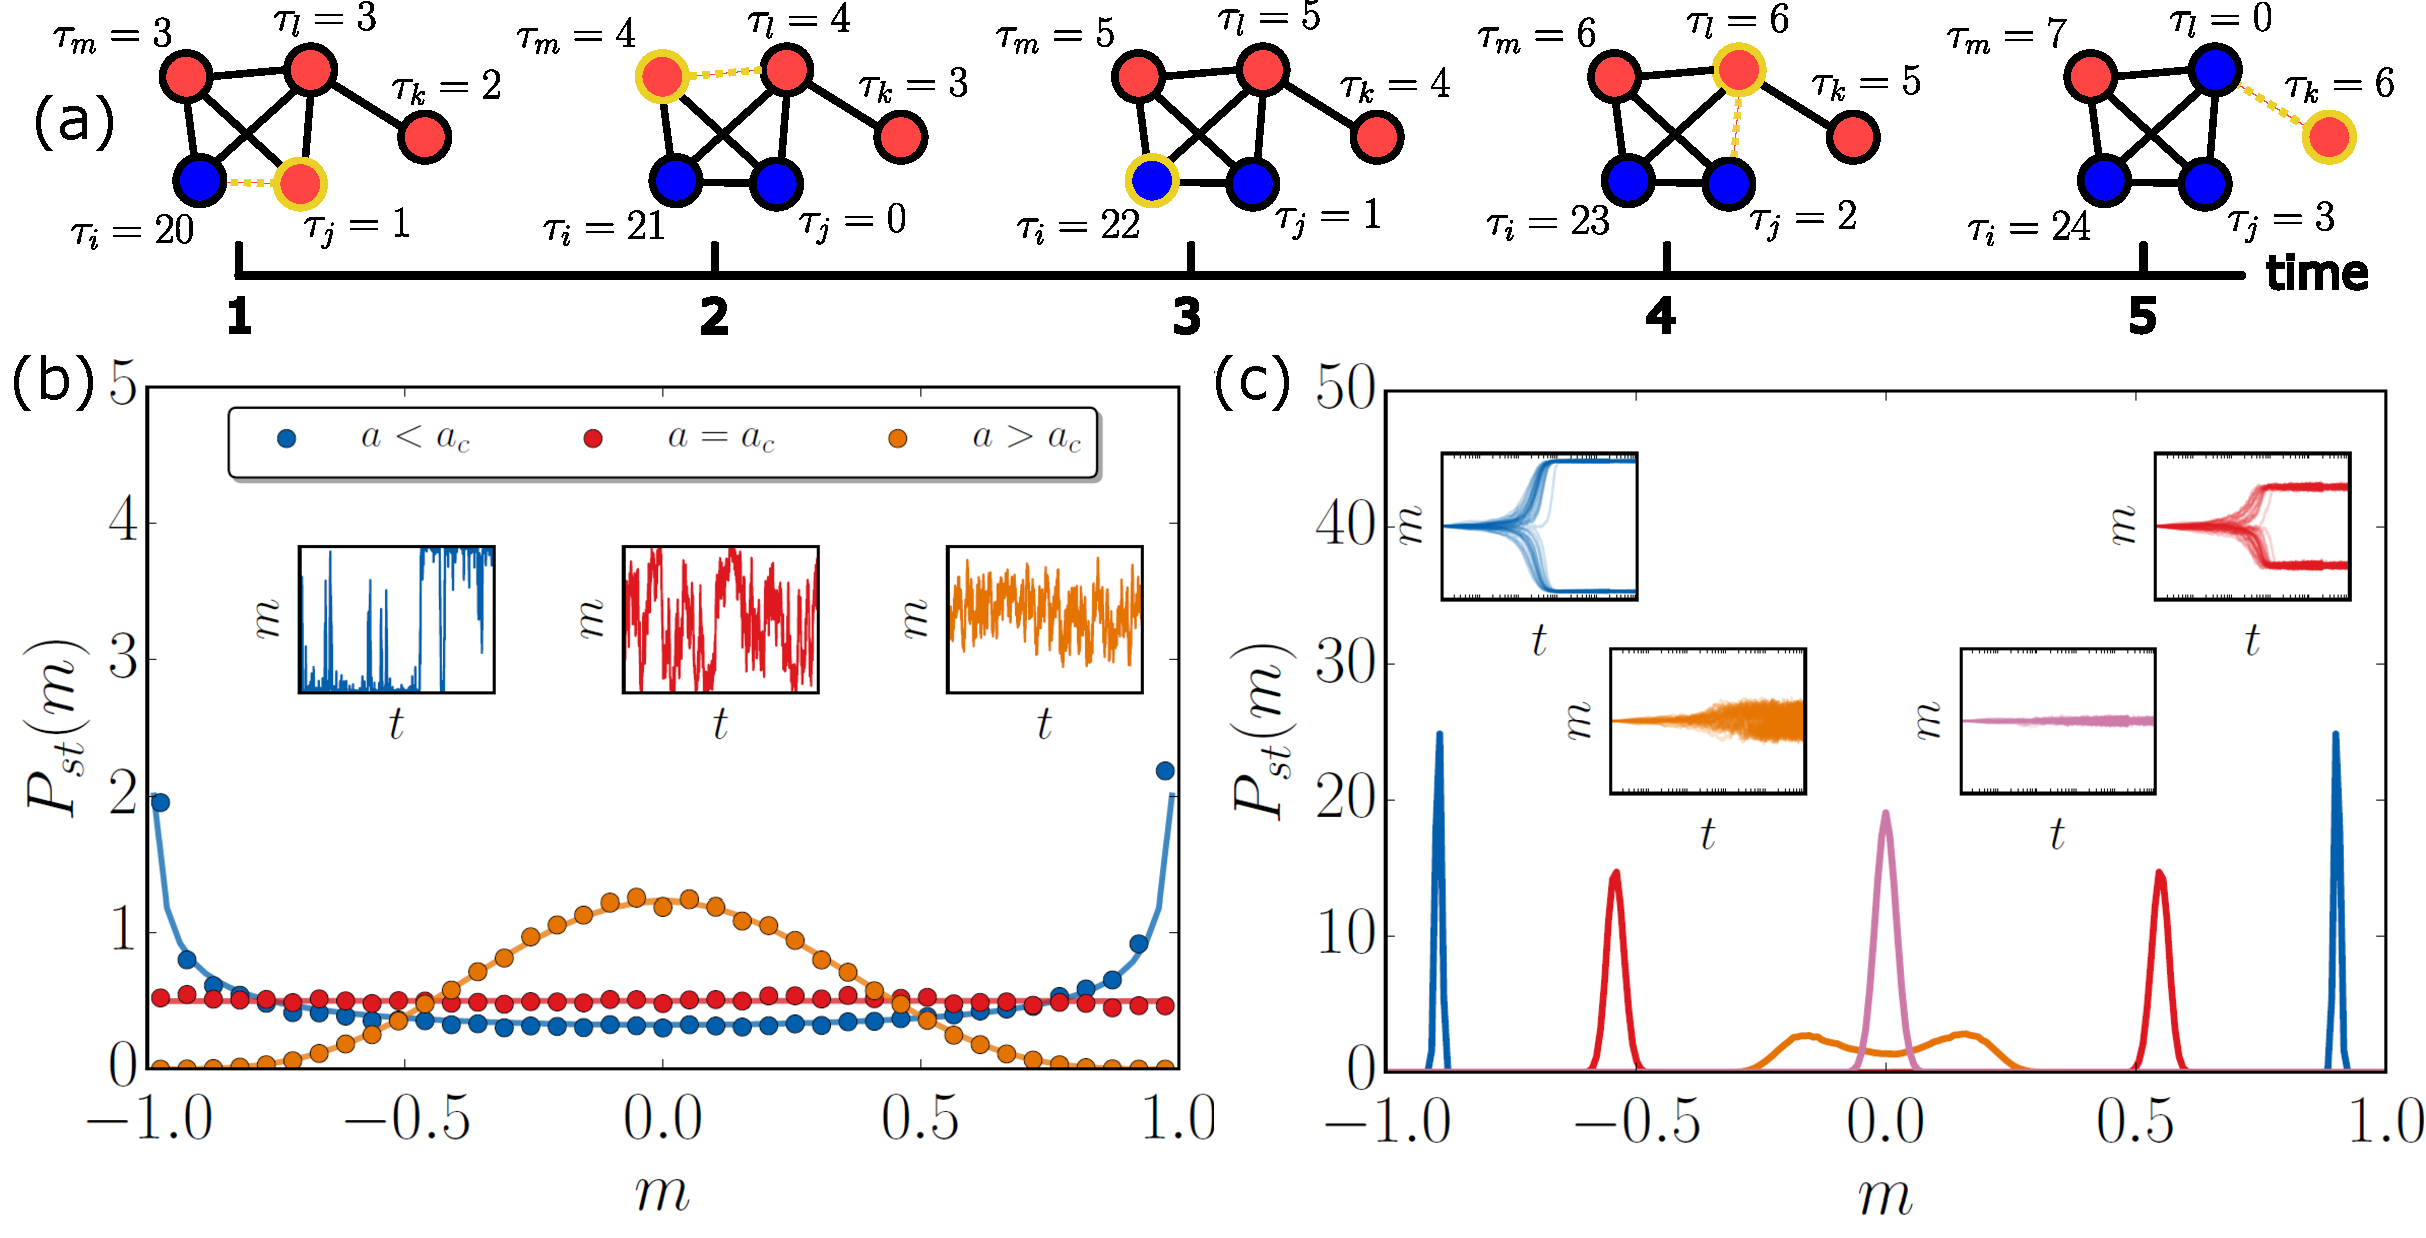
\includegraphics[width=\textwidth]{Figs/Introduction/aging_plot.pdf}
    \caption[Aging in the Voter model]{\textbf{(a)} Schematic representation of the evolution of the Voter model with aging. The node highlighted in yellow is the one attempting to activate and change state (copying the neighbour via the dashed yellow link). \textbf{(b)} Stationary probability density function (pdf) of the magnetization in the three different regimes. Points come from simulations, solid lines are the theoretical curves. The insets show one typical trajectory of the dynamics, in each of the regimes. \textbf{(c)} Stationary pdf for the noisy voter model with aging, in the different regimes. The insets show 50 trajectories of the magnetization. (from Ref. \cite{artime-2017}).}
    \label{fig:aging_pdf}
\end{figure}

To be clear, the aging mechanism is a non-Markovian effect that consists of an activation function that modifies the transition rates between states. This activation function depends on the time since the last transition, and it is a way to include bursty dynamics in the individuals' attempts to interact with others. This activation function is build such that probability of an individual to interact with another individual decreases with the time since the last interaction, even though there are studies that also account for anti-aging mechanisms (probability to interact increases) \cite{peralta-2020,chen-2020}.

The motivation behind the aging mechanism is to capture the tendency of individuals to stick to their previous beliefs or habits, a common feature in human behavior \cite{granovetter-1973}, and this attachment balances the memory-less and purely rational considerations of traditional models \cite{granovetter-1985}.

From the temporal interactions point of view, the aging mechanism is a way to include bursty dynamics in the individuals' attempts to interact with others (an activity-driven model). In this case, the probability of an individual to interact with another individual decreases with the time since the last interaction. It has been shown that the aging mechanism is able to produce the inter-event time distributions observed in empirical data \cite{fernandez-gracia-2011}, given a proper choice of the activation function.

\subsection{\label{sec:Aging in pairwise interactions} Aging in pairwise interactions}

Aging effects have been already shown to modify drastically the dynamics in the Voter model, a popular framework for exploring consensus formation in statistical physics and social dynamics. Counterintuitively, while aging can decelerate microdynamics by making state changes less frequent as agents' states age, it can accelerate macrodynamics, thus shortening the time required for the system to reach consensus. This phenomenon, observed across different network topologies, highlights the complex role of temporal elements in dynamic systems \cite{Stark2008,fernandez-gracia-2011, perez-2016, perez-2016,boguna-2014}.

In terms of stability, systems incorporating aging exhibit a tendency toward reaching stable configurations more swiftly compared to their non-aging counterparts. The persistence of the majority state, reinforced by aging, contributes to this stabilization, making aging a significant factor in determining the system's equilibrium state \cite{peralta-2020}. Furthermore, aging modifies the nature of the phase transition in the noisy Voter model. Specifically, it transforms a finite-size discontinuous transition between ordered and disordered phases into a continuous transition that falls into Ising universality class \cite{artime-2018}.

Moreover, this mechanism promotes longer persistence of the current majority state, thereby limiting the influence of fluctuating minority opinions over time and demonstrating a robust method for maintaining stability within a system \cite{peralta-2020}. These insights elucidate the complex interactions between temporal dynamics and system behaviors, offering a richer understanding of how consensus and order emerge in social and physical systems.

Regarding to models of multiple pairwise interactions or higher-order interactions, the aging implications are still an open question and it is a topic of current research. For the specific case of the noisy majority vote model \cite{chen-2020}, the aging mechanism is able to modify the critical point of the disordered-ordered phase transition. Further research is needed to understand the joint effect of aging and multiple interactions.